\chapter[MC event generation]{Understanding theory predictions via Monte-Carlo event generation}
\label{chap:MC}

Although we have nowadays a very elegant and complete theoretical description of particle physics, is not always evident how to translate this theory in actual predictions, to compare with measurements. Moreover, on the case of hadronic colliders, as the LHC, it's even more difficult due to the particularities of strong interaction. On this subject, a set of tools and approaches have been developed in order to be able to make accurate predictions from theory that could be directly researched for on the experiments, as CMS or ATLAS for example. In the present chapter, we describe such tools and formalisms and a set of studies comparing the predictions these tools to data. 

\section{Mote-Carlo simulations}
\label{sec:MC}

The Monte-Carlo simulations use random numbers and large samplings to calculate mathematical quantities in complex configurations, as integrals or probabilities. The typical example is on how to calculate the integral of a one-dimensional function. One can throw several random coordinates pair in the Cartesian plane and count how many of them are under the function. Then the integral of the function will be proportional to the fraction of points under the curve to the total thrown points. Larger the number of points, closer the estimation to the real value. An illustration of the procedure can be seen in figure~\ref{fig:mc_int}.

\begin{figure}[!Hhtbp]
  \begin{center}
    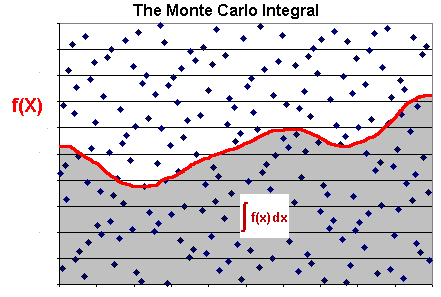
\includegraphics[width=0.6\textwidth]{figs/mc_integral.png}
    \caption{Integration using Monte-Carlo methods}
    \label{fig:mc_int}
  \end{center}
\end{figure}

A similar method is used to simulate proton-proton collisions. This simulation is used to generate ``random'' events and to calculate quantities, as the cross section, for a given physical process. Each event represent the final state of a collision, i.e. the set of particles produced from the collision and seen by a detector. Such simulations comprehend different stages: first, the partonic processes making reference to the interaction between the partons inside the proton; second, the hadronization of the particles produce from parton interactions; and third, the simulation of the interaction between the hadrons (from second step) and the detector material. Such events are used to evaluate predictions from theory in the frame of a specific experiment. Whereas the hadronization and detector simulation are well-known physical processes, new theories predictions rely basically on the partonic level, where the fundamental interaction processes take part.

\subsection{Parton simulation}
\label{sec:parton}

The parton model was initially proposed by Richard Feynman in 1969, as a method to understand collisions of non-fundamental particles. The model consider a non-fundamental particle, as a proton or a neutron, composed of a given number of point-like fundamental particles. When a collision occur the point-like particles inside have a major probability to scatter. For example, when an electron is fired against a proton the most of the interactions will between the electron and the fundamental components of the proton, $u$ and $d$ quarks. This ``hard'' components are called \textit{valence} quarks. Surrounding them there are the \textit{sea} quarks and gluons.

However, as the energy of the collision increases the probability to scatter a sea component, quark or gluon, increases. In addition, even if the valence quarks of a proton are the $u$ and $d$ quarks, heavier quarks can appear in the sea, as the $b$, $c$ or $s$ quarks. The probability to interact with a component, valence or sea, is described by parton distribution function, commonly called PDF. A PDF $f\equiv f(x,Q^{2})$ represent the number density of a given quark or gluon as a function of the energy scale $Q^{2}$ and the fraction of momentum carried by the parton $x$. The determination of a PDF is done via a fit of large data samples from experiments specifically designed to test the inner structure of nucleons. The DIS (Deep Inelastic Scattering) experiment at SLAC (Stanford Linear Accelerator Center), in California, United States, first probed the existence of partonic structure inside nucleons using leptons as probes scattered against nucleons. Another important experiment was the HERA accelerator at DESY in Hamburg, Germany, which used electrons to study the inner structure of protons.

In figure~\ref{fig:MSTW} is shown the Martin-Stirling-Thorne-Watt~\cite{Martin:2009iq} (MSTW) PDF for two energy scales. The MSTW PDF is one of the experimental fits combining data from DIS and HERA. In this PDF can be seen that $u$ and $d$ quarks carry the most of the momentum of the proton. The rest of the momentum is spread mainly over a huge amount of gluons and some, less probable, sea quarks as $\bar{u}, \bar{d}$ or $c$ and $s$. One important feature is that the composition of the proton changes depending on the energy scale. At $Q^{2}= 10\, GeV^{2}$ there is no $b$-quark in the proton while at $Q^{2}= 10^{4}\, GeV^{2}$ there is a non-negligible probability to find it in the proton.

\begin{figure}[!Hhtbp]
  \begin{center}
    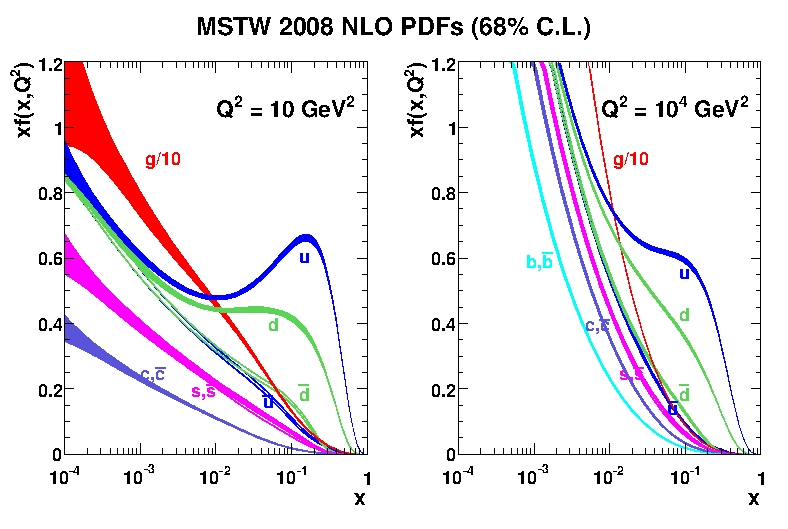
\includegraphics[width=0.9\textwidth]{figs/mstw2008nlo68cl_allpdfs.jpg}
    \caption{Martin-Stirling-Thorne-Watt proton PDF for $Q^{2}= 10\, \text{GeV}^{2}$ [left] and $Q^{2}= 10^{4}\, \text{GeV}^{2}$ [right]. From~\cite{Martin:2009iq}}
    \label{fig:MSTW}
  \end{center}
\end{figure}

Two other important PDF fits are CTEQ~\cite{Nadolsky:2008zw} and NNPDF~\cite{Ball:2010de}. Together with MSTW, they are the most used PDF sets in the CMS experiment for MC production. 

For the hard process, the differential cross section can be written as,

\begin{eqnarray}
  \label{eq:DiffXS}
  d\sigma_{ij\rightarrow lm} & = & \left( \int_{0}^{1}\int_{0}^{1}f_{i}(x_{i},Q^{2})f_{j}(x_{j},Q^{2})dx_{i}dx_{j} \right) \nonumber \\  
 & \times & \frac{d^{3}p_{l}}{(2\pi)^{2}2E_{l}}\frac{d^{3}p_{m}}{(2\pi)^{2}2E_{m}}\delta^{4}\left( p_{i}+p_{j}-p_{l}-p_{m} \right) \nonumber \\  
 & \times & |\mathcal{M}_{ij\rightarrow lm}|^{2}
\end{eqnarray} where $f_{i,j}$ correspond to the PDF's of the initial partons. $\mathcal{M}_{ij\rightarrow lm}$ is the matrix element of the process which is the part of the S-matrix that contains the amplitude of the process, and modules the transition from the initial to the final state~\cite{opac-b1131978}. The matrix element could account effectively for all processes mediating the transition from the initial to the given final state, but in practice it is calculated only including a given number of processes. The calculation can achieve different levels, usually tree level or Leading Order (LO), but modern calculation could arrive, depending on the process, to one loop or Next-to-Leading-Order (NLO) or even two loops the  Next-to-Next-to-Leading-Order (NNLO). This limit depends exclusively on the feasibility of the theoretical calculations. In figure~\ref{fig:LOpNLO} is shown an example of a leading order plus its corresponding NLO diagrams for a fermion scattering.

\begin{figure}[!Hhtbp]
  \begin{center}
    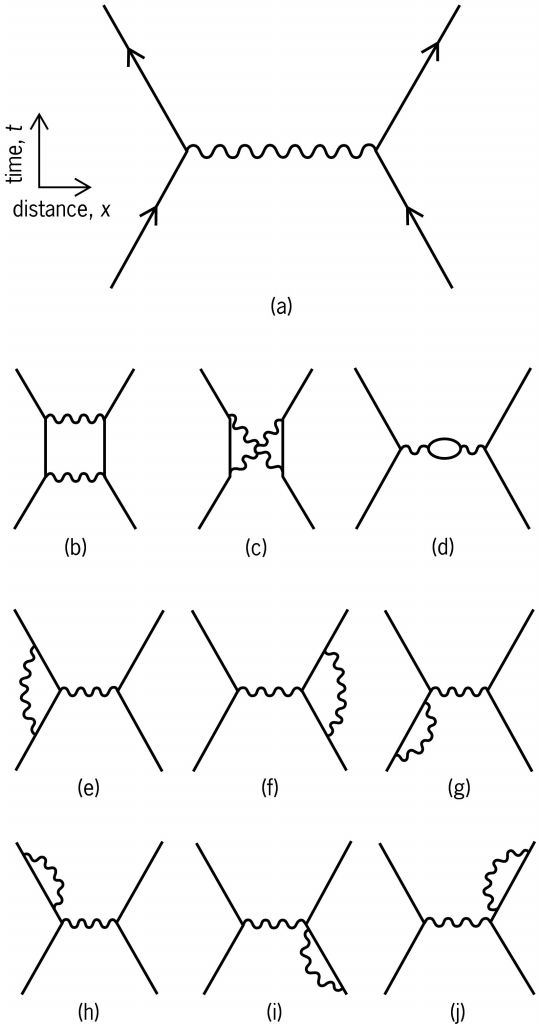
\includegraphics[width=0.7\textwidth]{figs/Feynman_diagrams.jpg}
    \caption{LO (a) and NLO (b)-(j) processes contributing to fermions scattering}
    \label{fig:LOpNLO}
  \end{center}
\end{figure}

\subsection{Hadron simulation}
\label{sec:hadron}

Description of how partons can't be seen free but inside hadrons.

\begin{figure}[!Hhtbp]
  \begin{center}
    
\includegraphics[width=0.3\textwidth]{figs/CMSlogo.png}
    \caption{Graphical representation of hadronization process of partons resulting from a proton-proton collision.}
    \label{fig:Hadr}
  \end{center}
\end{figure}
%\begin{TOINCLUDE}Figure to illustrate to hadronization process\end{TOINCLUDE}

\subsection{Detector simulation}
\label{sec:detector}

Description on how the detector is simulated, and how the detector response is simulated to be the closest possible to data with Geant4.

\section{Tools}
\label{sec:tools}

\subsection{Matrix-element generators}
\label{sec:ME}

Description of calculations performed by the MadGraph.

\subsection{Hadron generators}
\label{sec:Had}

Hadronization procedures performed by Pythia and Herwig.

\section{Validation on data}
\label{sec:val}

Description of validation process of known processes against different MC predictions.

\begin{figure}[!Hhtbp]
  \begin{center}
    
\includegraphics[width=0.3\textwidth]{figs/CMSlogo.png}
    \caption{$W+$jets simulated by several MC generators compared to data}
    \label{fig:WVal}
  \end{center}
\end{figure}

\begin{figure}[!Hhtbp]
  \begin{center}
    
\includegraphics[width=0.3\textwidth]{figs/CMSlogo.png}
    \caption{$Z+$jets simulated by several MC generators compared to data}
    \label{fig:WVal}
  \end{center}
\end{figure}

Observed differences on the measured top pt and MC predictions.

\begin{figure}[!Hhtbp]
  \begin{center}
    
\includegraphics[width=0.3\textwidth]{figs/CMSlogo.png}
    \caption{Data MC comparison of ratio of normalized diff cross section as function of the $p_{T}$ of the top.}
    \label{fig:WVal}
  \end{center}
\end{figure}
%\begin{TOINCLUDE}Plot of W+jets and Z+jets comparison between data and MC for a set of different generators. Plot on top pt to briefly introduce tpo pt reweighting\end{TOINCLUDE}